\section{Immune Network Theory}

\begin{frame}
\Huge \textbf{Immune Network Theory}
\large {Shi,Haixin}
\end{frame}

\begin{frame}{Immune Network Theory}{Jerne's idiotypic network hypothesis}
  \begin{itemize}
  \item \large{
    Immunologists in the early 1970's were in the process of discovering a wealth of information about how the immune system worked.
  }
  \item \large{
    Jerne's network hypothesis was a radical innovation, which states that the regulation of the adaptive immune system involves interactions between V regions.
  }
  \end{itemize}
\end{frame}

\begin{frame}{Immune Network Theory}{Jerne's idiotypic network hypothesis}
   \begin{itemize}
   \item \large
    Jerne introduced three terms:
    \begin{itemize}
    \item
      \large{\textcolor{red}{epitope} (antigenic determinant): the part of an antigen that is recognized by the immune system.}
    \item
      \large{\textcolor{red}{idiotope}: the unique set of antigenic determinants (epitopes) of the variable portion of an antibody.}
    \item
      \large{\textcolor{red}{paratope} (antigen-binding site): is a part of an antibody which recognizes and binds to an antigen.}
    \end{itemize}
  \end{itemize}
\end{frame}

\begin{frame}{Immune Network Theory}{Dualisms}
   \begin{itemize}
   \item \large
    two main kinds of cells:
    \begin{itemize}
    \item
      \large{T cells}
    \item
      \large{B cells}
    \end{itemize}
   \item \large
    two main kinds of interactions:
    \begin{itemize}
    \item
      \large{stimulation}
    \item
      \large{suppression}
    \end{itemize}
  \end{itemize}
\end{frame}

\begin{frame}{Immune Network Theory}{Jerne's model of the network}
  \begin{itemize}
  \item \large
     The network was proposed by Jerne in 1973.
  \end{itemize}
  \par
  \centering
    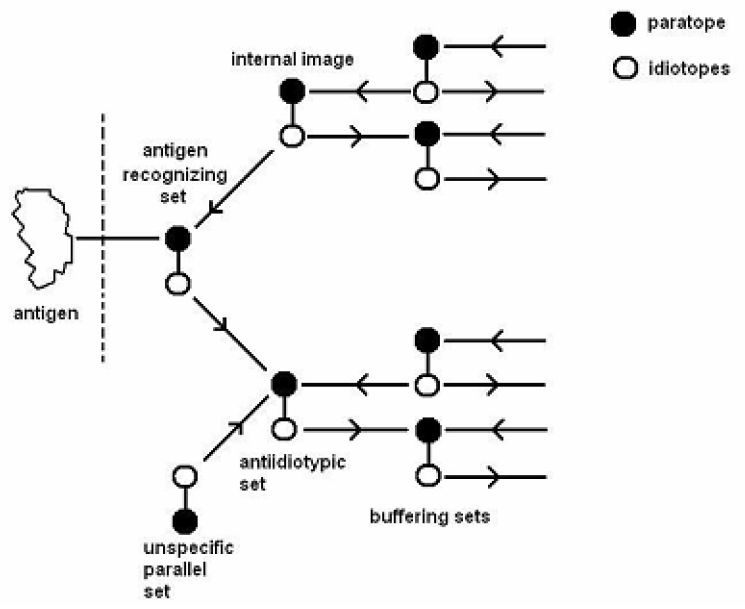
\includegraphics[scale=0.5] {img/network_model_jerne.png}
  \par
\end{frame}

\begin{frame}{Immune Network Theory}{The first mathematical model}
  \begin{itemize}
  \item \large
     The formula describes the dynamics of a typical clone consisting of L cells (lymphocytes):
  \end{itemize}
  \begin{equation} \large{
     \frac{dL}{dT}= \alpha -\beta L+\sum_{i=1}^{N}\varphi (E_{i},K_{i},t)-L\sum_{j=1}^{n}\psi (I_{j},K_{j},t)}
  \end{equation}
\end{frame}

\begin{frame}{Immune Network Theory}{Limitations of the Jerne model}
  \begin{itemize}
  \item \large
   While Jerne's model was a huge conceptual advance, he candidly recognized it's
   limitations:
   \begin{columns}[c] 
    \column{.45\textwidth} 
    \begin{itemize}
    \item \large{(a)Simplicity}
    \item \large{(b)Scope}
    \item \large{(c)Predictions}
    \item \large{(d)Resolution of Paradoxes}
    \end{itemize}
    \column{.55\textwidth} 
    \begin{itemize}
    \item \large{(e)Mechanistic basis}
    \item \large{(f)Rigour}
    \item \large{(g)Robustness}
    \item \large{(h)Aesthetics}
    \end{itemize}
    \end{columns}
  \end{itemize}
\end{frame}

\begin{frame}{Immune Network Theory}{The Richter theory}
  \begin{itemize}
  \item \large
     The network was thus simplified from Jerne's two-dimensional network to a one dimensional chain.
  \end{itemize}
  \par
  \centering
    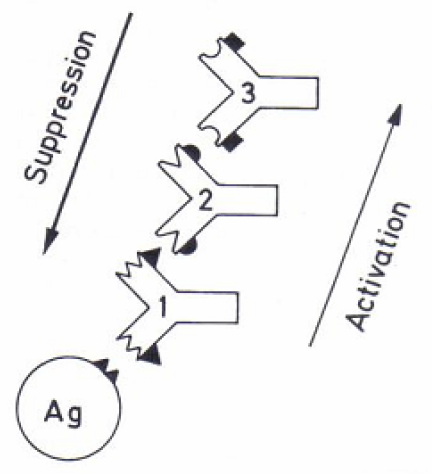
\includegraphics[scale=0.5] {img/network_model_richter.png}
  \par
\end{frame}

\begin{frame}{Immune Network Theory}{Modes of response}
  \begin{itemize}
  \item \large
     Low dose tolerance in the Richter model.
  \end{itemize}
  \par
  \centering
    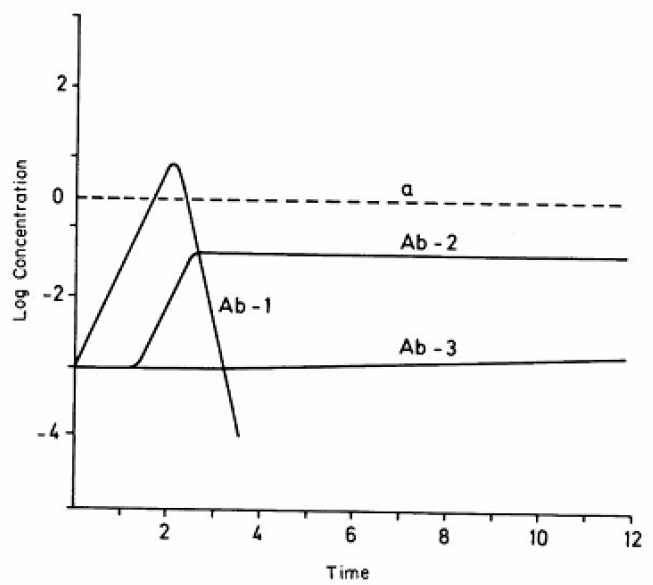
\includegraphics[scale=0.5] {img/low_dose_tolerance.png}
  \par
\end{frame}

\begin{frame}{Immune Network Theory}{Modes of response}
  \begin{itemize}
  \item \large
     The immune response in the Richter model.
  \end{itemize}
  \par
  \centering
    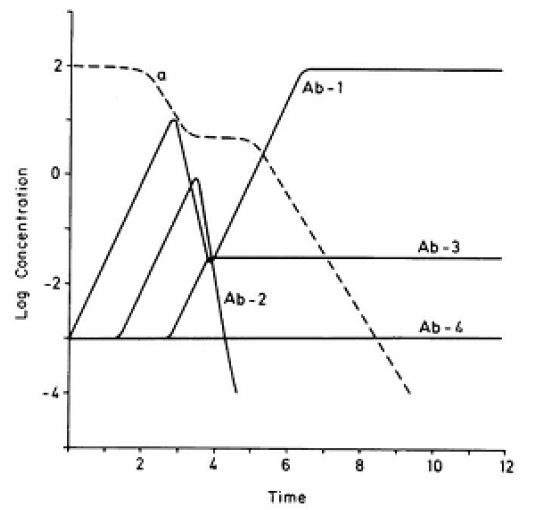
\includegraphics[scale=0.5] {img/immune_response.png}
  \par
\end{frame}

\begin{frame}{Immune Network Theory}{Modes of response}
  \begin{itemize}
  \item \large
     High dose tolerance in the Richter model.
  \end{itemize}
  \par
  \centering
    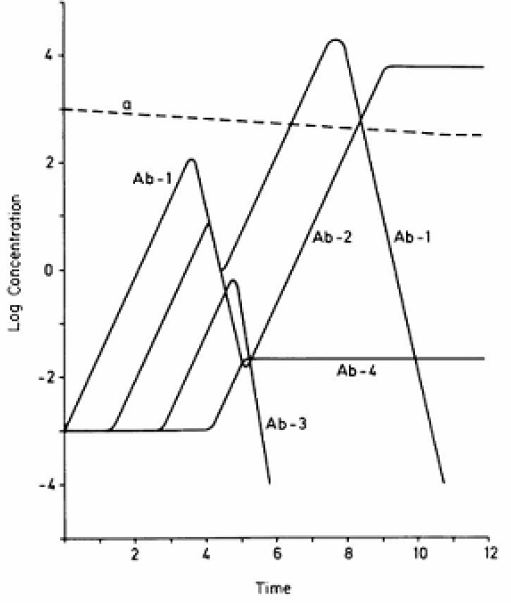
\includegraphics[scale=0.5] {img/high_dose_tolerance.png}
  \par
\end{frame}

\begin{frame}{Immune Network Theory}{Modes of response}
  \begin{itemize}
  \item \large
    The improved network model which adds inhibitory interactions.
  \end{itemize}
  \par
  \centering
    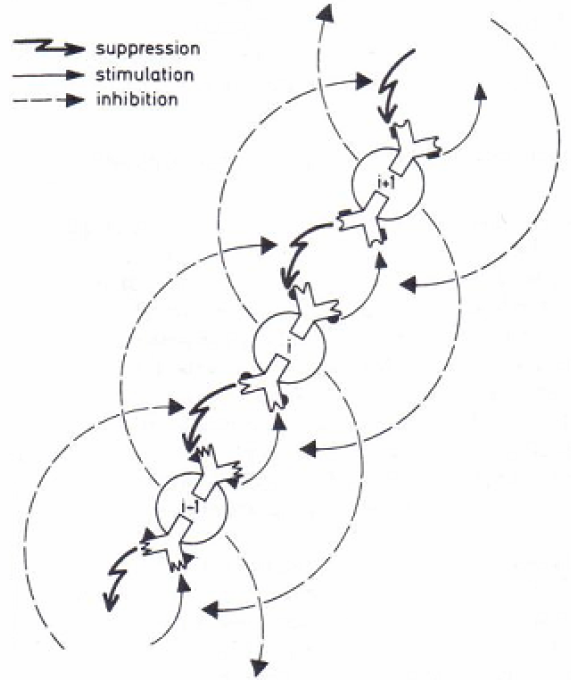
\includegraphics[scale=0.4] {img/Improved_network_model.png}
  \par
\end{frame}

\begin{frame}{Immune Network Theory}{Richter's mathematical model}
  \begin{itemize}
  \item \large
    Richter translated the above ideas into differential equations, and pictures above can be obtained by integrating his equations:
  \end{itemize}
  \begin{equation} \large{
    \frac{dS_{i}}{dt}=\frac{1}{\tau _{b}}f(S_{i-1},S_{i},S_{i+1})S_{i}-\frac{1}{\tau _{d}}g(S_{i-1},S_{i},S_{i+1})S_{i}}
  \end{equation}
\end{frame}

\begin{frame}{Immune Network Theory}{Achievements of the Richter theory}
  \begin{itemize}
  \item \large{
    It showed that Jerne's network concept could be reduced to manageable proportions.
  }
  \item \large{
    The Richter theory showed that there are three basic types of specific interactions which are important for such models - stimulation, inhibition (blocking) and elimination (killing).
  }
  \item \large{
    It illustrated a potential importance of thresholds in stabilizing the immune system.
  }
  \end{itemize}
\end{frame}

\begin{frame}{Immune Network Theory}{The symmetrical network theory}
  \begin{itemize}
  \item \large
    The symmetrical network theory incorporates symmetric interactions between idiotypes and antiidiotypes.
  \end{itemize}
  \par
  \centering
    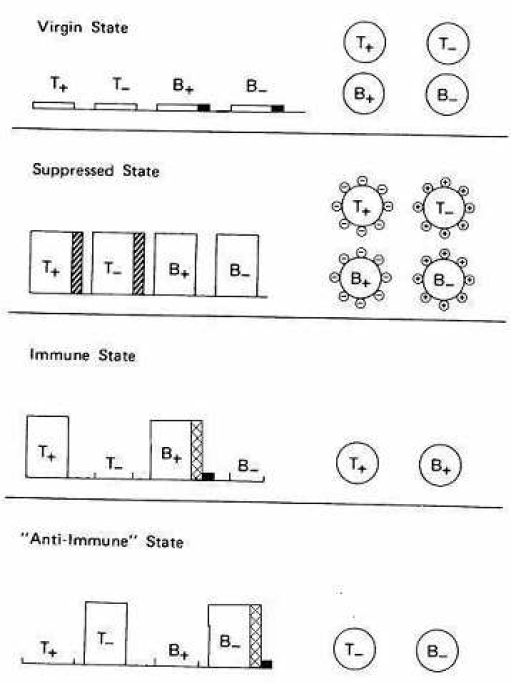
\includegraphics[scale=0.40] {img/symmetrical_network_theory.png}
  \par
\end{frame}

\begin{frame}{Immune Network Theory}{The environmental detection algorithm}
  \begin{itemize}
  \item \large{
    The movement direction of robot:
  }
  \end{itemize}
  \par
  \centering
    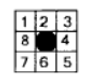
\includegraphics[scale=0.8] {img/movement_direction.png}
  \par
  \begin{itemize}
  \item \large{
    The antigen information of robot:
  }
  \end{itemize}
  \begin{equation} \large{
     g_{i}=\frac{1}{(k_{1}\cdot expense+k_{2}\cdot occupy+k_{3}\cdot gain+1)}}
  \end{equation}
\end{frame}

\begin{frame}{Immune Network Theory}{The environmental detection algorithm}
  \begin{itemize}
  \item \large{
    The interaction between robotic antibodies:
  }
  \end{itemize}
  \par
  \centering
    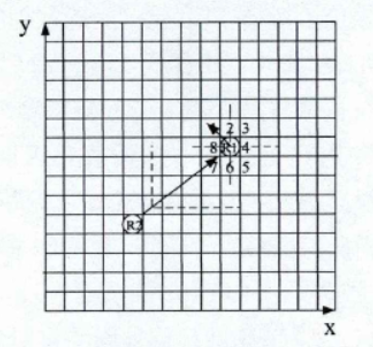
\includegraphics[scale=0.6] {img/immune_network_force_diagram.png}
  \begin{equation} \large{
     \overline{R_{2}R_{1}}=\overline{(x_{2}-x_{1})(y_{2}-y_{1})}}
  \end{equation}
\end{frame}

\begin{frame}{Immune Network Theory}{The environmental detection algorithm}
  \centering
    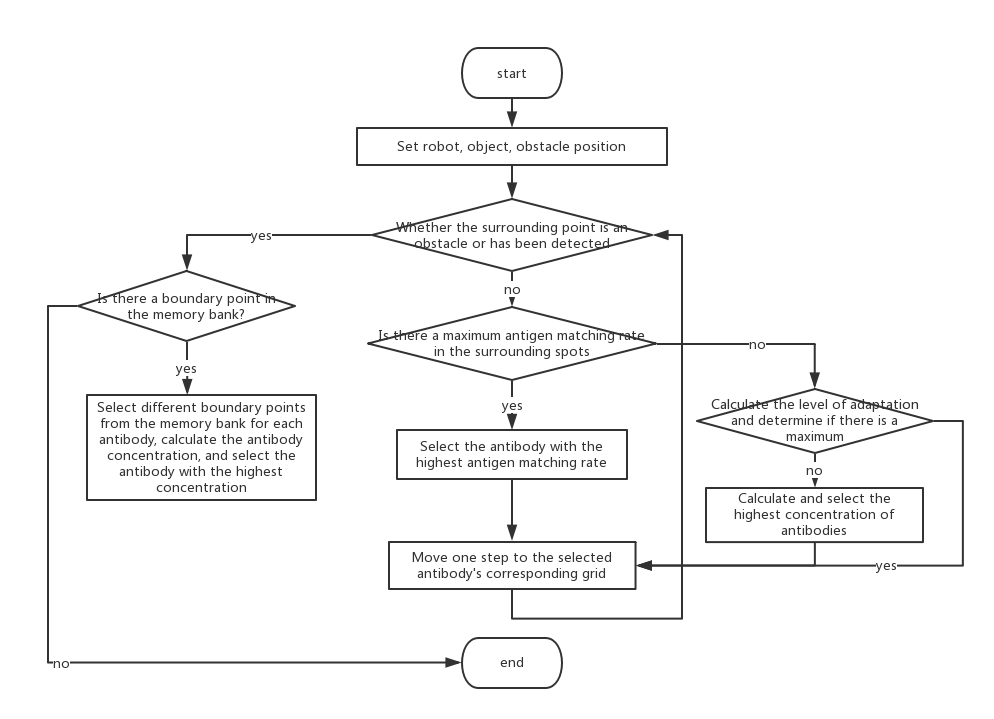
\includegraphics[scale=0.30] {img/immune_network_flowchat.png}
\end{frame}

\begin{frame}{Immune Network Theory}{The environmental detection algorithm}
  \centering
    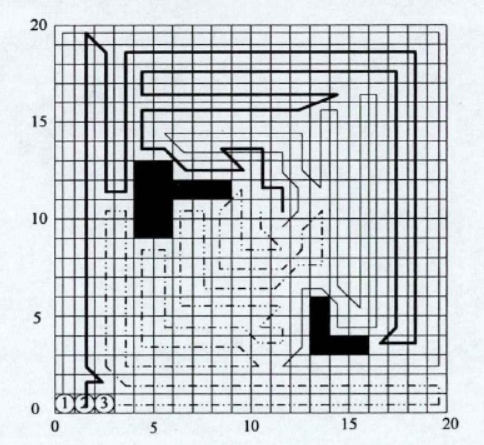
\includegraphics[scale=0.70] {img/immune_network_route_map.png}
\end{frame}


